\section{Hardware}
\lipsum[4-8]
\begin{figure}
\centering
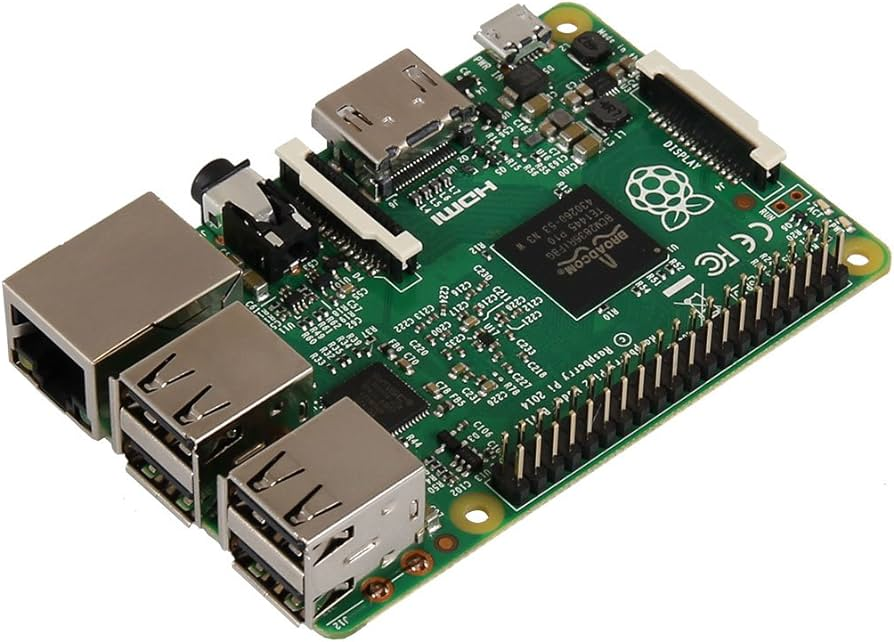
\includegraphics[width=0.5\textwidth]{images/raspimg.jpg}
\caption{Raspberry Pi 4 Model B}

\end{figure}

\section{Software Overview}

\subsection{ESRGAN for Image Super-Resolution}
\begin{figure}[H]
    \centering
    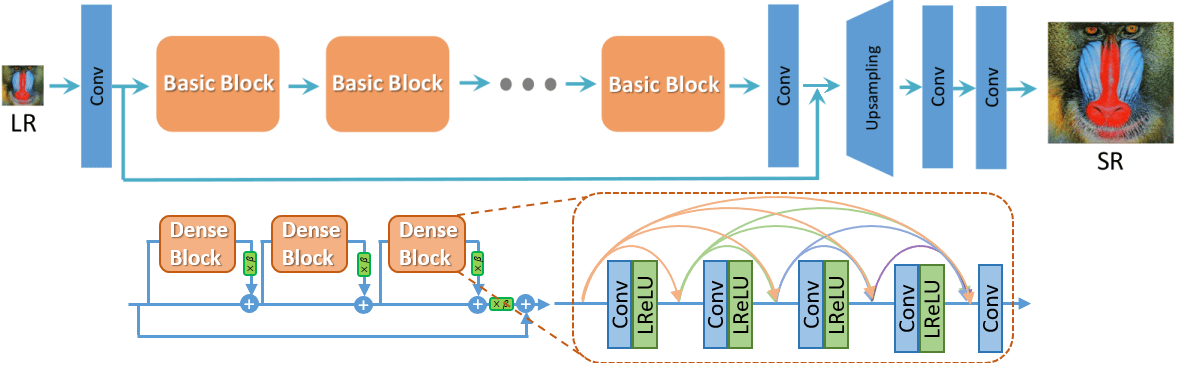
\includegraphics[width=0.85\linewidth]{images/esrganarchi.png}
    \caption{ESRGAN Architecture with Residual-in-Residual Dense Blocks (RRDB)}
    \label{fig:esrgan}
\end{figure}
ESRGAN introduced by Wang \emph{et al.} in 2018 [1], improves upon SRGAN by employing a deep generator built from Residual‑in‑Residual Dense Blocks (RRDB) without batch normalization. Each RRDB combines multiple convolutional layers, local dense connections, and global residual links to capture complex image features. The generator upsamples low‑resolution inputs (e.g.\ 820×616 pixels) by a factor of 4× to high‑resolution outputs (e.g.\ 3280×2464 pixels). The discriminator is relativistic, estimating the probability that a real image is more realistic than a generated one, which enhances stability and visual fidelity. ESRGAN further integrates a perceptual loss based on high‑level VGG features computed before ReLU activations, preserving fine textures and brightness consistency. This design enables ESRGAN to produce photorealistic details, as demonstrated by its victory in the PIRM2018 SR Challenge [1].

In our UAV system, images captured onboard with a Raspberry Pi USB Camera are retrieved post‑flight. ESRGAN runs on a ground PC to upscale extracted frames, recovering critical details (e.g.\ building outlines, vegetation patterns) necessary for accurate land use classification in the Kathmandu region.

\subsection{Comparison of Super-Resolution Models}
We compare ESRGAN with earlier SR approaches:

\begin{table}[H]
\centering
\renewcommand{\arraystretch}{1.2}
\setlength{\tabcolsep}{6pt}
\begin{tabular}{@{} l l p{3cm} p{3cm} p{3cm} @{}}
    \toprule
    \textbf{Model} & \textbf{Year} & \textbf{Architecture} & \textbf{Strengths} & \textbf{Weaknesses} \\
    \midrule
    SRCNN   & 2014 & 3-layer CNN & Simple, fast & Overly smooth outputs [2] \\
    FSRCNN  & 2016 & CNN + deconv & Efficient, higher PSNR [2] & Limited texture detail \\
    EDSR    & 2017 & Deep ResNet & High PSNR, faster [3] & Less perceptual quality \\
    ESRGAN  & 2018 & GAN + RRDB & Realistic textures, sharp edges [1] & Computationally intensive \\
    \bottomrule
  \end{tabular}
  \caption{Comparison of Super-Resolution Models}
\label{tab:sr_models}
\end{table}


\subsection{Land Use Classification}
Land use classification from UAV imagery entails categorizing pixels or patches into classes such as forest, agriculture, water, and urban. Common approaches include:
\begin{itemize}
  \item \textbf{Convolutional Neural Networks (CNNs)}: End‑to‑end models (e.g.\ U‑Net, ResNet, EfficientNet) that learn spatial hierarchies directly from upscaled images [4].
  \item \textbf{Random Forest (RF)}: Ensemble of decision trees trained on raw pixels or derived indices, robust to overfitting and effective for moderate datasets [2,4].
  \item \textbf{Support Vector Machine (SVM)}: Kernel‑based classifier suitable for moderate‑sized, well‑separated classes [2,4].
\end{itemize}
A hybrid approach often combines CNN feature extractors with RF or SVM classifiers, leveraging deep networks for hierarchical feature learning and traditional ML for robust classification when labeled data is limited.

\subsection{Software}
The software pipeline integrates the following tools and libraries:
\begin{itemize}
  \item \textbf{OpenCV}: For image/frame extraction, filtering, and geometric transformations [5].
  \item \textbf{NumPy \& SciPy}: Core numerical and array operations for preprocessing.
  \item \textbf{scikit-learn}: Implements RF and SVM classifiers, data splitting, scaling, and evaluation utilities [6].
  \item \textbf{TensorFlow \& PyTorch}: Deep learning frameworks for ESRGAN and CNN implementation. PyTorch (BasicSR toolkit) eases experimentation [7], while TensorFlow (TF‑Hub ESRGAN) supports scalable deployment [8].
  \item \textbf{GDAL/Rasterio}: For handling geo-referenced imagery and aligning with regional GIS data [9].
\end{itemize} 


\subsection{Dataset}

\textbf{1. Kathmandu Land Use Datasets}

Region-specific datasets used for land use classification in Kathmandu:

\begin{itemize}
  \item \textbf{Nepal National Land Cover Dataset}: Annual land-cover maps (2000–2022) from Landsat imagery via Google Earth Engine, covering forests, agriculture, water, and built-up areas[10].
  \item \textbf{Kathmandu City Land Use Shapefiles}: Urban land use polygons (residential, commercial, parks) for Kathmandu Metropolitan City (2011) from ICIMOD[11].
  \item \textbf{OpenStreetMap Polygons}: Land-use tags for Kathmandu accessible through the Humanitarian Data Exchange[12].
\end{itemize}

\textbf{2. Image Super-Resolution Datasets}

Datasets used to train and evaluate ESRGAN and other super-resolution models:

\begin{itemize}
  \item \textbf{DIV2K}: A large-scale dataset designed for image super-resolution, consisting of 1000 high-resolution images and their corresponding low-resolution counterparts. Suitable for training deep SR models.
  \item \textbf{Set5 and Set14}: Benchmark datasets commonly used for evaluating the performance of super-resolution models. While smaller in size, they are widely adopted for quantitative comparisons.
\end{itemize}

These datasets provide essential ground truth for training and validating both our land use classification pipeline and image super-resolution models.

